\chapter{Multiagenten Strategien}
\label{chap:explorative}

Dieses Kapitel widmet sich der Untersuchung emergenter Verhaltensweisen zweier konkurrierender Agentenpopulationen in einer Multi-Agent-Reinforcement-Learning-Umgebung. Die Agenten repräsentieren Jäger und Beute, wodurch sich sowohl ihre individuellen Strategien, als auch die Dynamik zwischen den Populationen analysieren lassen.

\section{Methodik}

Für die Simulation kommt das Multi-Agent-Reinforcement-Learning-Framework \textit{PettingZoo} \cite{Terry_PettingZoo_Gym_for} zum Einsatz, welches eine standardisierte Schnittstelle zur Erstellung und Integration eigener Umgebungen bietet. Ziel ist die Analyse emergenter Verhaltensmuster in einem Szenario mit zwei voneinander lernenden Agentengruppen. Dabei wird ein dezentraler Lernansatz verfolgt, bei dem jede Population unabhängig ihre Policy optimiert.

\paragraph{Environment}
Das Environment bildet eine Überlebenssimulation in einer zweidimensionalen, kontinuierlichen Welt ab. In dieser Simulation interagieren zwei Typen von Agenten miteinander: Jäger und Beute. Beide Typen verfügen über dieselben Aktionsmöglichkeiten und strukturellen Eigenschaften und haben das Ziel, so lange wie möglich zu überleben. Bewegung und Interaktionen kosten Energie, welche die Agenten wiederherstellen müssen: Beute regenerieren ihren Vorrat, indem sie Futter von den auf der Karte verteilten Feldern sammelen, während Jäger Energie gewinnen, wenn sie erfolgreich eine Beute erlegen. Wenn ihre Energie vollständig verbraucht ist, sterben die Agenten. Neben den Futterquellen existieren auf der Karte Hindernisse wie ein Fluss, der sich über die gesamte Karte erstreckt, sowie Steine, die die Agenten verschieben können. Zusätzlich gibt es ein Waldobjekt, das die Sicht der Agenten einschränkt, aber passierbar ist. Dieser Aufbau dynamischer Objekte soll das Entwickeln von Strategien und das Planen von Schritten motivieren. Das Environment ermöglicht außerdem Gruppeninteraktionen, bei denen sich beispielsweise Beuten gemeinsam gegen Jäger verteidigen oder Jäger gemeinsam Beuten angreifen. Diese Implementierung soll Teamstrategien und gemeinsames Handeln motivieren, indem gemeinsames überleben erleichtert wird.
\newpage
\begin{figure}[htbp]
\centering
\adjincludegraphics[
     width=0.9\linewidth,
     Clip={0 {0\height} 0 {0.1\height}} 
  ]{Bilder/marl.png}
\caption{Multiagenten Umgebung}
\label{fig:marl}
\end{figure}


\paragraph{Observationsraum}
Die eingesetzte Zustandsrepräsentation basiert auf einem rasterbasierten Sichtfeld, in dem diskrete Felder auf Kollisionen mit Objekten oder Agenten geprüft werden. Das Sichtfeld erstreckt sich über einen Halbkreis in die Blickrichtung des Agenten. Jeder Unterbereich in diesem Raster wird daraufhin kategorisiert und erhält einen nummerischen Wert, welcher die Art des Objektes kodiert, mit dem es kollidiert. Zusätzlich erhält der Agent Informationen über die eigene Blickrichtung, Geschwindigkeit, Energielevel und Alter.

\paragraph{Aktionsraum}
Die Agenten können zwischen den Aktionen \textit{Bewegen} und \textit{Angreifen} wählen, wobei jede Aktion mit einem eigenen Bewegungsvektor kombiniert ist. Dieser Bewegungsvektor gibt hierbei die Richtung und Stärke der Bewegung an, wobei eine \textit{Bewegung} eine höhere Maximaldistanz besitzt als ein \textit{Angriff}. Die Blickrichtung des Agenten wird anschließend in die resultierende Bewegungsrichtung angepasst, so dass der Agent immer in Laufrichtung blickt.

\paragraph{Modellaufbau}

Die entwickelte Modellarchitektur für die Agenten basiert auf einer Kombination aus einer Self-Attention-Komponente \cite{vaswani2023attentionneed}, einer rekurrenten Schicht, sowie mehreren spezialisierten Ausgabeköpfen. Der Eingabevektor wird zunächst durch eine Dense-Schicht projiziert. Anschließend werden die daraus resultierenden Merkmale durch einen Multihead-Attention-Mechanismus verarbeitet, um relevante Interaktionen innerhalb der Daten dynamisch hervorzuheben. Die zeitlichen Abhängigkeiten und Sequenzen werden mithilfe eines LSTM erfasst.

Aus dem LSTM-Output erfolgen drei separate Ausgabeköpfe zur Berechnung der Aktionen: Der erste Kopf berechnet die Bewegungsrichtung, ein weiterer verarbeitet die Angriffsrichtung analog. Der dritte Kopf entscheidet zwischen Bewegungs- und Angriffshandlung und nutzt dafür ein zweischichtiges Dense-Netzwerk mit Softmax-Ausgabe, die eine normierte Aktionsverteilung liefert. Zusätzlich existiert ein Value-Kopf, welcher den erwarteten kumulierten Ertrag schätzt.

Die Netzwerkstruktur mit Neuronenanzahl ist in Tabelle \ref{tab:neuronenanzahl_marl} dargestellt.

\begin{table}[htbp]
\centering
\caption{Neuronenanzahl pro Schicht}
\label{tab:neuronenanzahl_marl}
\begin{tabular}{lc}
\toprule
Schicht & Neuronenanzahl \\
\midrule
Dense & 256 \\
Multihead Attention & 256 (4 Köpfe) \\
LSTM & 256 \\
Move Direction Head Dense & 32 \\
Attack Direction Head Dense & 32 \\
Action Selection Head Dense & 32 \\
Value Head Dense & 32 \\
\bottomrule
\end{tabular}
\end{table}


\paragraph{Belohnungsstruktur und Training}
Die Hauptbelohnung der Agenten orientiert sich an der Differenz des aktuellen Energielevels im Vergleich zum vorherigen Zeitschritt. Eine positive Energieveränderung wird belohnt, das Verbrauchen von Energie wird bestraft. Zusätzlich erhalten die Agenten positive Rewards für das Annähern an Nahrung, während Stillstand oder Kollisionen mit Hindernissen negative Belohnungen nach sich ziehen. Diese Struktur soll implizit das Verhalten „Jagen vs.\ Flüchten“ fördern. Die Agenten erhalten außerdem eine steigende Belohnung, je länger sie überleben. Ein evolutionärer Mechanismus greift ebenfalls: Agenten mit höherer Überlebensdauer pflanzen sich fort und vererben ihre Policy (mit leichten Mutationen) an die nächste Generation. Dadurch soll ein Selektionsdruck zugunsten vorteilhafter Strategien entstehen – analog zu biologischer Evolution. Wie in natürlichen Systemen setzen sich anpassungsfähige Verhaltensweisen über Generationen hinweg durch, während weniger erfolgreiche Strategien verschwinden. Dieser Ansatz fördert langfristig robuste und effiziente Problemlösungen, auch in komplexen und dynamischen Umgebungen.

\section{Ergebnisse}

Trotz der konzeptionell vielseitigen Anlage zeigten die Tests nur begrenzte Lernerfolge, wobei die Probleme hauptsächlich auf die Struktur der Belohnung sowie die Gestaltung des Observations- und Aktionsraums zurückzuführen sind. Die Reward-Struktur erwies sich als zu komplex und nicht ausreichend differenziert, um den Agenten konsistente und eindeutige Lernsignale zu liefern. Beispielsweise führten zufällige Bewegungen eines Jäger-Agenten häufig dazu, dass er kontinuierlich positive Belohnungen erhielt, während eine Beute-Agentin negative Belohnungen erhielt, unabhängig vom tatsächlichen Verhalten. Diese Dynamik führte regelmäßig zu einem Policy Collapse, bei dem suboptimale Verhaltensweisen verstärkt und alternative Strategien systematisch vernachlässigt wurden.

Auch in Tests ohne Reward-Shaping blieben Lernerfolge vollständig aus: Die Agenten verhielten sich über mehrere Trainingsläufe hinweg zufällig und nicht adaptiv. Selbst bei vereinfachten Belohnungsstrukturen, die lediglich Nahrungssuche und Jagen belohnten, konnten die Agenten keine nachhaltigen Fortschritte erzielen.

Abbildung ~\ref{fig:reward} illustriert exemplarisch den Reward-Verlauf eines Jäger- und eines Beute-Agenten. Nach einer anfänglichen Verbesserung folgte eine instabile Phase mit stark schwankenden Rewards. Diese Phase ist typisch für Policy-Collapse-Situationen und entstand durch chaotische und lokale Interaktionen zwischen den konkurrierenden Agentengruppen.

\begin{figure}[h]
\centering
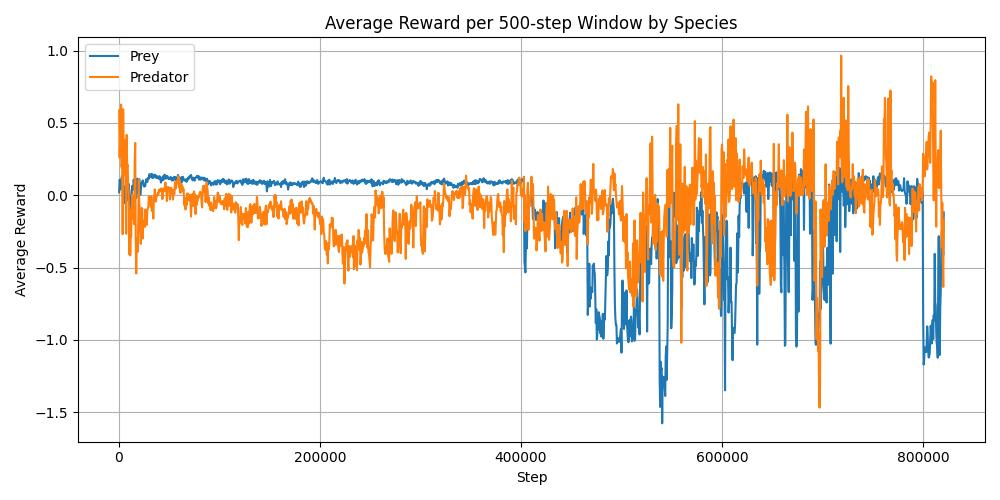
\includegraphics[width=0.9\linewidth]{Bilder/collapse.jpg}
\caption{Policy Collapse bei Jäger und Beute}
\label{fig:reward}
\end{figure}

\section{Diskussion}

Die unzureichenden Lernergebnisse lassen sich auf mehrere kritische Faktoren zurückführen. Die komplexe und wenig differenzierte Reward-Struktur verhinderte klare und konsistente Lernsignale. Widersprüchliche und unklare Belohnungen verwirrten die Agenten und resultierten in ineffizienten Verhaltensmustern.

Darüber hinaus erschwerte die verwendete Zustandsrepräsentation mittels rasterbasierter Beobachtung ohne explizite Positions- oder Richtungsinformationen eine klare und konsistente Interpretation der Umgebung. Die inkonsistente Wahrnehmung, hervorgerufen durch sprunghafte Änderungen der Blickrichtung und kategoriale Kodierung, verstärkte diese Problematik zusätzlich. Zusätzlich verschärften Belohnungskomponenten, die das Annähern an Nahrung oder das Entfernen von Gegnern belohnten, die Problematik. Wenn mehrere Objekte gleichzeitig wahrnehmbar waren, entstanden widersprüchliche Signale. So konnten Bewegungen in verschiedene Richtungen gleichermaßen positiv bewertet werden, was dazu führte, dass die Agenten oft in einem ziellosen Hin-und-Her-Verhalten zwischen zwei relevanten Objekten verharrten, anstatt zielgerichtete Strategien zu entwickeln.

Ein weiterer kritischer Punkt war die getrennte Behandlung von Bewegungs- und Angriffsentscheidungen, die aufgrund der doppelten Aktionsauswahl häufig zu redundanten oder widersprüchlichen Handlungen führte. Diese strukturellen Schwächen verhinderten die Entwicklung robuster und generalisierbarer Strategien.

Zukünftige Untersuchungen sollten daher eine vereinfachte und differenzierte Belohnungsstruktur, eine stabilere und konsistentere Zustandsrepräsentation sowie eine integrierte Aktionsauswahl berücksichtigen, um nachhaltige Lernprozesse zu fördern.
